\medskip

	\begin{enumerate}
		\item \begin{enumerate}
	\item Résolvons, dans $[0~;~1]$, l'équation demandée :

$ \begin{aligned}[t]  f(x) = x &\iff 2x \e^{-x} = x\\
&\iff 2x \e^{-x} - x = 0\\
&\iff x(2\e^{-x}-1) = 0\\
&\iff x = 0 \quad \text{ ou } \quad 2\e^{-x} - 1 = 0\\
&\iff x = 0 \quad \text{ ou } \quad 2\e^{-x} = 1\\
&\iff x = 0 \quad \text{ ou } \quad \e^{-x} = \dfrac{1}{2}\\
&\iff x = 0 \quad \text{ ou } \quad -x = \ln\left(\dfrac{1}{2}\right) \\
&\iff x = 0 \quad \text{ ou } \quad x = \ln(2)
\end{aligned}$

Or, 0 et ln(2) sont deux réels dans [0~;~1] (en effet, la stricte croissance de ln sur $\R^{*+}$ donne: \quad $1 < 2 < \e \implies 0 < \ln(2) < 1$).

L'équation a donc deux solutions dans $ [0~;~1] $ : 0 et ln(2).

	\item $f$ est dérivable sur $ [0~;~1] $, en tant que composée et produit de fonctions qui pourraient être définies et dérivables sur $\R$ :

$\forall x \in [0 ; 1],\quad f'(x) = 2 \times \e^{-x} + (2x) \times (-\e^{-x})
 = (2 - 2x)\e^{-x} = 2(1 -x)\e^{-x}$.

On arrive donc à l'expression demandée.

		\item On sait que la fonction exponentielle est à valeurs strictement positives sur $\R$. On a :\quad $f(0) = 2\times 0 \e^{-0} = 0$ \quad et \quad $f(1) = 2\times 1\e^{-1} = 2\e^{-1}$.

On peut donc établir le tableau de variations de la fonction :

\begin{center}
	\begin{tikzpicture}
		\tkzTabInit[lgt=3]{$x$/0.8,signe de 2/0.8,signe de $(1-x)$/0.8,signe de $\e^{-x}$/0.8,signe de $f'(x)$/0.8,variations de $f$/2}{0,1}
	\tkzTabLine{t,+,t}
		\tkzTabLine{t,+,z}
		\tkzTabLine{t,+,t}
		\tkzTabLine{t,+,z}
		\tkzTabVar{-/0,+/$2\e^{-1}$}
	\end{tikzpicture}
			\end{center}
		\end{enumerate}

		\item 
		\begin{enumerate}
			\item \emph{Initialisation :} Calculons $u_1$. $u_1 = f(u_0) = f(0,1) = 2\times 0,1\e^{-0,1} \approx 0,18$.

On constate que l'inégalité est vraie pour $n = 0$, on a bien : \quad $ 0\leqslant u_0 < u_1 \leqslant 1$.

\smallskip

\emph{Hérédité :} Pour un entier naturel $k$ donné, on suppose que l'inégalité \quad $ 0\leqslant u_k < u_{k+1} \leqslant 1$\quad est vraie.

Montrons que l'inégalité sera vraie au rang suivant :

Par hypothèse de récurrence on a :

$ \begin{aligned}[t] 0\leqslant u_k < u_{k+1} \leqslant 1
&\implies f(0) \leqslant f(u_k) < f(u_{k+1}) \leqslant f(1)\\
&\hphantom{\implies}\quad \text{car $f$ est strictement croissante sur }[0 ; 1]\\
&\implies 0 \leqslant u_{k+1 } < u_{k+2} \leqslant 2\e^{-1}\\
&\hphantom{\implies}\quad \text{car $f$ est la fonction de récurrence de la suite  } (u_n)\\
&\implies 0 \leqslant u_{k+1 } < u_{k+2} \leqslant 1\\
&\hphantom{\implies}\quad \text{car } 2\e^{-1} \approx 0,74 < 1\\		\end{aligned}$


Ainsi, la véracité de l'inégalité est héréditaire.

\smallskip

\emph{Conclusion :} L'inégalité est vraie au rang 0, et sa véracité est héréditaire pour tout entier naturel, donc, en vertu du principe de récurrence, on a :

$\forall n \in \N,\quad 0 \leqslant u_{n} < u_{n+1} \leqslant 1$.

		\item On a notamment :
\begin{itemize}
\item $\forall n \in \N,\quad u_{n} < u_{n+1}$. \quad La suite $(u_n)$ est donc (strictement) croissante.
\item $\forall n \in \N,\quad 0 \leqslant u_{n}\leqslant 1$. \quad La suite $(u_n)$ est donc bornée par 0 et 1.
\end{itemize}

La suite étant croissante et majorée, on en déduit qu'elle est donc convergente, vers une limite $\ell$ vérifiant $0 \leqslant \ell \leqslant 1$.
		\end{enumerate}

		\item La suite $(u_n)$ est une suite convergente, définie par récurrence par la relation $u_{n+1} = f(u_n)$, où la fonction $f$ est continue (car dérivable) sur $ [0 ; 1] $, intervalle qui contient la limite $\ell$ de la suite.

D'après le théorème \og du point fixe \fg{}, on en déduit que la limite ne peut être qu'une solution de l'équation $f(x) = x$ dans l'intervalle $ [0~;~1] $.

D'après la question \textbf{1. a.}, cette équation n'a que deux solutions dans $ [0 ; 1] $ : 0 et ln(2), or la suite est (strictement) croissante, donc minorée par son premier terme : $u_0 = 0,1$, donc la limite ne saurait être inférieure à 0,1 : la possibilité d'avoir $\ell = 0$ est donc écartée, et finalement, l'unique valeur possible pour $\ell$ est donc $\ln(2)$.

La suite $(u_n)$ converge donc vers ln(2).

	\item \begin{enumerate}
		\item La suite $\left(u_n\right) $ est croissante et converge vers ln(2), donc elle est majorée par $ln (2)$.

On a donc :\quad $\forall n \in \N, \quad u_n \leqslant \ln(2) \implies \ln(2) - u_n \geqslant 0$.

Pour tout entier naturel $n$, la différence $\ln(2) - u_n$ est bien positive.

		\item Un terme de la suite $(u_n)$ sera donc toujours une valeur approchée par défaut de $\ln(2)$. Si on veut que la valeur approchée soit à $ 10^{-4} $ près, cela signifie que la différence entre $u_n$, la valeur approchée, et $\ln(2)$ doit être inférieure ou égale à $ 10^{-4} $.

On va donc explorer les termes consécutifs de la suite $(u_n)$ tant que 

$\ln(2) - u_n > 0,0001$, de sorte que la boucle s'interrompra dès que la différence deviendra inférieure ou égale à $ 10^{-4} = 0,0001 $.

Le script ci-dessous convient (à condition d'avoir importé les fonctions \texttt{exp} et \texttt{log} qui est la fonction logarithme népérien,  de la librairie \texttt{math}, au préalable).

On a dans ce corrigé ajouté les deux lignes qui rendent le programme exécutable

	\begin{center}
		\ttfamily
		\begin{tabularx}{10cm}{|X|}\hline
			from math import exp\\
			from math import log as ln\\
			def seuil():\\
			\quad n=0\\
			\quad u=0.1\\
			\quad while ln(2) - u {\red >} 0.0001:\\
			\quad \quad n=n+1\\
			\quad \quad u={\red 2*u*exp(-u)}\\
			\quad return(u,n)\\ \hline
		\end{tabularx}
	\end{center}

\emph{Remarque :} on peut aussi importer la constante d'Euler de la librairie maths et utiliser une variante :
			\texttt{from math import e } en lieu et place de la première ligne et
			\texttt{u={\red 2*u*e**(-u)}} ou \texttt{u={\red 2*u/(e**u)}} pour l'avant dernière.
			\item $n = 11$	
		\end{enumerate}
	\end{enumerate}
